Esta seção descreve o pipeline proposto, ilustrado na Figura~\ref{fig:method}, estruturado em três etapas: (i) materiais, (ii) pré-processamento e (iii) extração de características e treinamento.

\begin{figure}[h]
    \centering
    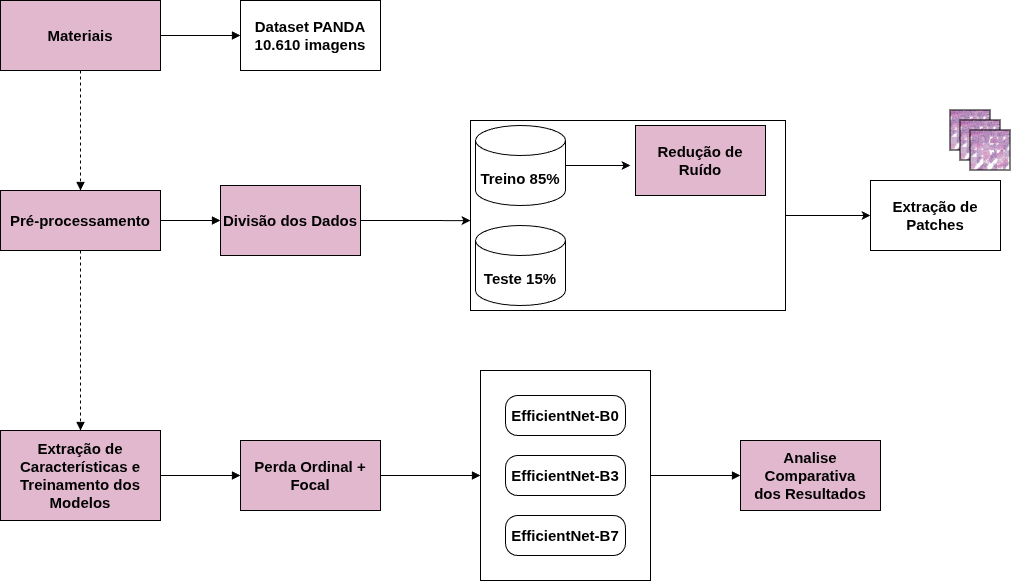
\includegraphics[width=0.9\linewidth]{images/method-semish.png}
    \caption{Pipeline proposto.}
    \label{fig:method}
\end{figure}

\subsection{Materiais}
\label{sub:data}

Foi utilizada a base de dados PANDA (\textit{Prostate Cancer Grade Assessment}), composta por aproximadamente 10.616 WSIs de biópsias prostáticas \cite{ref-panda2020}, coletadas em dois centros médicos - \textit{Radboud University Medical Center} e \textit{Karolinska Institute} - introduzindo variabilidade institucional representativa da prática clínica. As imagens são anotadas com escore e grau de Gleason. O conjunto apresenta distribuição desigual entre as seis classes ISUP (0 a 5), com maior concentração nas classes ISUP 0 e 1, além de ruídos como artefatos visuais e inconsistências de rotulação (Figura~\ref{fig:distribuicao-isup}).

\begin{figure}[htb]
	\centering
	\includegraphics[width=0.9\textwidth,height=0.25\textheight]{"images/distribuição ISUP"}
	\caption{Distribuição das amostras da base PANDA por grau ISUP.}
	\label{fig:distribuicao-isup}
\end{figure}

\subsection{Pré-processamento}

Os dados foram divididos em conjuntos de treinamento e teste. Na sequência, aplicou-se redução de ruído baseada em entropia e, por fim, extração de \textit{patches}.

\textbf{Redução de ruído por entropia.} Quatro modelos EfficientNet (B0-B3) foram usados para calcular a entropia de Shannon e quantificar a incerteza das predições \cite{ali2023entropy}. A entropia média dos quatro modelos foi calculada por amostra, e o percentil superior de 10\% formou um banco de amostras candidatas a ruído. Avaliaram-se quatro cenários (remoção de 0\%, 20\%, 50\% e 100\% dessas amostras), sendo a remoção de 20\% (180 amostras) a que produziu melhor desempenho.

\textbf{Extração de \textit{patches}.} Como as WSIs são de alta dimensionalidade e o tecido ocupa apenas parte da lâmina, foram geradas novas imagens por reorganização em \textit{patches}. Avaliaram-se configurações 5×5, 6×6 e 7×7; a configuração 6×6 (36 \textit{patches}, 1536×1536 px) foi selecionada por equilibrar cobertura tecidual, qualidade e eficiência computacional.

\subsection{Extração de características e treinamento}

A EfficientNet-B0 foi utilizada como modelo-base para ajuste de hiperparâmetros (\textit{fine-tuning} com 150 camadas descongeladas, taxa de aprendizado $3\times10^{-4}$, \textit{dropout} 0,4, 50 épocas, otimizador Adam). Essa configuração foi então estendida às EfficientNet-B3 e B7.

A função de perda baseline (\textit{Binary Cross-Entropy}) foi substituída por uma formulação híbrida que reflete a natureza ordinal do ISUP. Cada grau $k \in \{0,\dots,5\}$ é codificado como vetor binário cumulativo ($k$ primeiros elementos iguais a 1), e a perda ordinal é aplicada a cada limiar, impondo penalização proporcional à distância entre classes. Para mitigar o desbalanceamento, a perda ordinal foi combinada à \textit{Focal Loss} \cite{lin2017focal} ($\gamma = 2{,}0$, $\alpha = 0{,}25$), priorizando amostras de maior incerteza diagnóstica. O desempenho foi avaliado por \textbf{acurácia} e pelo \textbf{Kappa Quadrático Ponderado} ($\kappa_{\text{quad}}$), com intervalos de confiança estimados via bootstrap não paramétrico (1.000 reamostragens, IC de 90\%).
